% Portfolio presentation — Hanif Edma
% Light theme matching hanifedma.com/portfolio. Compile with:
%   latexmk -pdf portfolio_presentation.tex
% One idea per slide: Background (skills + education), then each project as
% Image -> Objective -> Outcome/Contribution -> Technical skills.
\documentclass[aspectratio=169,11pt]{beamer}

\usepackage[T1]{fontenc}
\usepackage[utf8]{inputenc}
\usepackage[sfdefault]{roboto}      % Roboto (the site's font) — works with pdfLaTeX
\usepackage{graphicx}
\usepackage{xcolor}
\usepackage{tikz}
\usepackage{hyperref}

% --- standard Beamer theme (navy header/footer bars) ---
\usetheme{Madrid}
\usecolortheme{whale}
\usefonttheme{professionalfonts}
\setbeamertemplate{navigation symbols}{}
\setbeamertemplate{frametitle continuation}{}  % no "(cont.)" on wrapped titles
\setbeamerfont{frametitle}{size=\normalsize}   % smaller frame titles (default is \large)

% footer bar without the author/website box (keep title + frame number)
\setbeamertemplate{footline}{%
  \leavevmode%
  \hbox{%
  \begin{beamercolorbox}[wd=.333333\paperwidth,ht=2.25ex,dp=1em,center]{author in head/foot}%
  \end{beamercolorbox}%
  \begin{beamercolorbox}[wd=.333333\paperwidth,ht=2.25ex,dp=1em,center]{title in head/foot}%
    \usebeamerfont{title in head/foot}\insertshorttitle%
  \end{beamercolorbox}%
  \begin{beamercolorbox}[wd=.333333\paperwidth,ht=2.25ex,dp=1em,right]{date in head/foot}%
    \usebeamerfont{date in head/foot}%
    \insertframenumber{} / \inserttotalframenumber\hspace*{2ex}%
  \end{beamercolorbox}}%
  \vskip0pt%
}

% --- palette for chips & links ---
\definecolor{accent}{HTML}{2563EB}
\definecolor{textmain}{HTML}{1A1A1A}
\definecolor{textsec}{HTML}{404040}
\definecolor{cardbg}{HTML}{F3F4F6}
\definecolor{borderc}{HTML}{E5E7EB}

\hypersetup{colorlinks=true, urlcolor=accent, linkcolor=accent}
\urlstyle{same}

% pull images from the website's optimized assets and the local figures folder
\graphicspath{{../portfolio/}{figures/}}

% title metadata -- drives the title page and the footer bar
\title[Portfolio]{Portfolio}
\subtitle{Background, Research \& Engineering Projects}
\author[Hanif Edma]{Hanif Edma}
\institute[hanifedma.com]{\url{https://hanifedma.com/portfolio_presentation}}
\date{}

% tag pills (matching the website's chips)
\newcommand{\chip}[1]{\tikz[baseline=(c.base)]\node[fill=cardbg, draw=borderc,
  rounded corners=2pt, inner xsep=4pt, inner ysep=2.5pt] (c) {\color{textsec}\small #1};\hspace{2pt}}
\newcommand{\chipaward}[1]{\tikz[baseline=(c.base)]\node[fill=cardbg, draw=borderc,
  rounded corners=2pt, inner xsep=4pt, inner ysep=2.5pt] (c) {\color{textmain}\small\bfseries #1};\hspace{2pt}}

% small uppercase section kicker (Research / Engineering Projects)
\newcommand{\kicker}[1]{{\color{accent}\bfseries\footnotesize\MakeUppercase{#1}}\par\smallskip}

% big accent heading for the per-slide part (Objective / Outcome / Technical skills)
\newcommand{\heading}[1]{{\color{textmain}\bfseries\Large #1}}

% left-aligned accent label for the combined Objective + Outcome slide
\newcommand{\blocklabel}[1]{\par{\color{textmain}\bfseries\large #1}\par\smallskip}

% link line: "Label: url"
\newcommand{\linkline}[2]{{\footnotesize #1: \url{#2}}}

% section suffix folded into the frame title: "Title — Section"
% (light weight, on the theme's coloured title bar)
\newcommand{\sectsuffix}[1]{\,{\normalfont\mdseries\,\textemdash\ #1}}

\begin{document}

% ---------- Title ----------
\begin{frame}[plain]
  \titlepage
\end{frame}

% ========================================================
% BACKGROUND
% ========================================================
\section{Background}

% --- Education ---
\begin{frame}{Background\sectsuffix{Education}}
  \vfill
  \begin{itemize}\setlength\itemsep{16pt}
    \item \textbf{Seoul National University of Science and Technology (SEOULTECH)}\\[2pt]
          {\small M.S., Electrical \& Information Engineering --- GPA 4.19 / 4.50}\\[1pt]
          {\small\color{textsec} Seoul, South Korea \,\textbullet\, Feb 2024 -- Aug 2026 (Expected) \,\textbullet\, Research Assistant}
    \item \textbf{Universitas Indonesia}\\[2pt]
          {\small B.S., Electrical Engineering --- GPA 3.61 / 4.00}\\[1pt]
          {\small\color{textsec} Depok, Indonesia \,\textbullet\, Aug 2019 -- Aug 2023}
  \end{itemize}
  \vfill
\end{frame}

% --- Technical skills (overview) ---
\begin{frame}{Background\sectsuffix{Technical Skills}}
  \begin{center}\small\color{textsec}
    Focus: Robotics (mobile robots) \,\textbullet\, Control \& Estimation \,\textbullet\, Electrical Engineering
  \end{center}
  \medskip
  \begin{itemize}\small\setlength\itemsep{7pt}
    \item \textbf{Control \& Estimation:} MPC / MPPI / MPCC, PID, LQR, Kalman Filter (KF/EKF), 2D SLAM, Motion Planning \& Trajectory Optimization
    \item \textbf{Machine Learning:} Gaussian Process (GP/SGP), Neural Networks, Imitation Learning, PyTorch \& TensorFlow (basic)
    \item \textbf{Programming \& Frameworks:} ROS1 / ROS2, C/C++, Python, MATLAB/Simulink, CasADi, Flutter, HTML/CSS/JS, OpenCV (basic)
    \item \textbf{Tools \& Platforms:} Gazebo, move\_base, Linux, Git, Docker
    \item \textbf{Hardware \& IoT:} NVIDIA Jetson, Raspberry Pi, Arduino, ESP32
  \end{itemize}
\end{frame}

% ========================================================
% RESEARCH
% ========================================================
\section{Research}

% ---------- GP-RAMPPI ----------
\begin{frame}{Performance-Enhanced Risk-Aware MPPI using Gaussian Process\sectsuffix{Research}}
  \vfill
  \begin{center}
    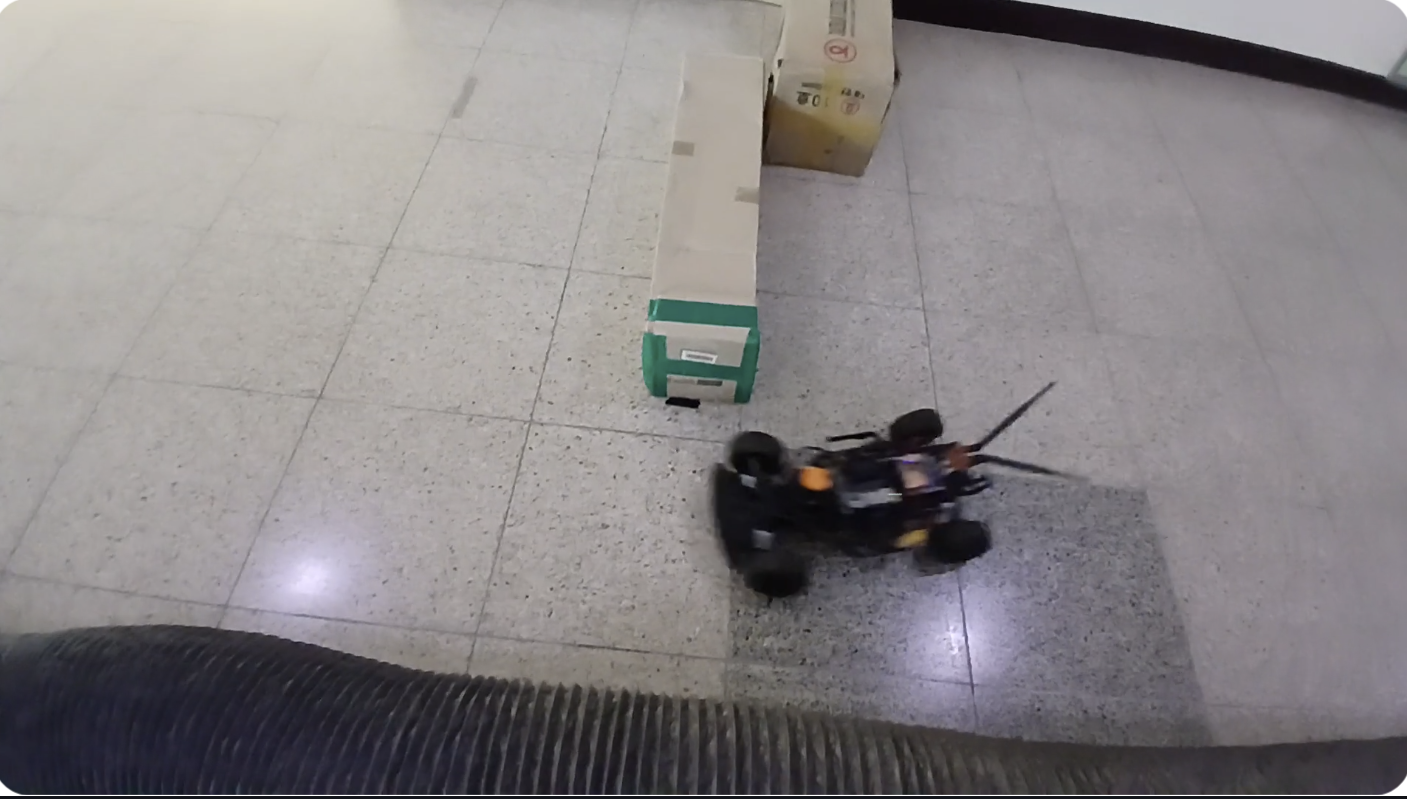
\includegraphics[width=\linewidth,height=0.72\textheight,keepaspectratio]{propose_rw_1stpaper.png}\\[8pt]
    {\scriptsize\color{textsec} Real-world run --- proposed method}
  \end{center}
  \vfill
\end{frame}

\begin{frame}{Performance-Enhanced Risk-Aware MPPI using Gaussian Process\sectsuffix{Research}}
  \vfill
  \begin{columns}[c]
    \begin{column}{0.47\textwidth}\centering
      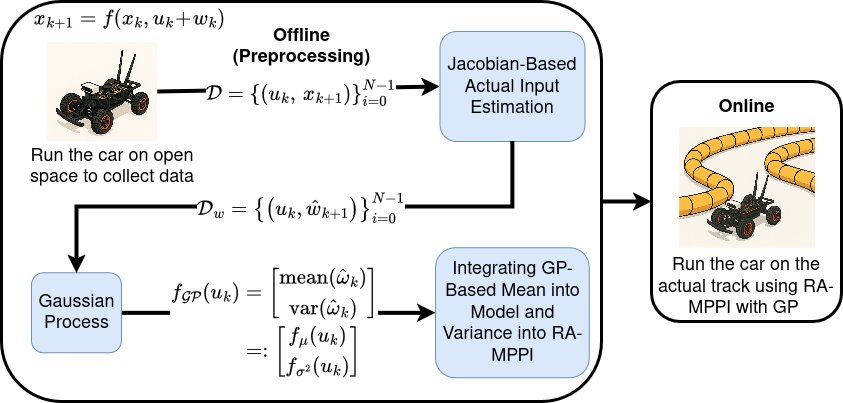
\includegraphics[width=\linewidth,height=0.6\textheight,keepaspectratio]{gpramppi.jpg}\\[8pt]
      {\scriptsize\color{textsec} Method framework}
    \end{column}
    \begin{column}{0.47\textwidth}\centering
      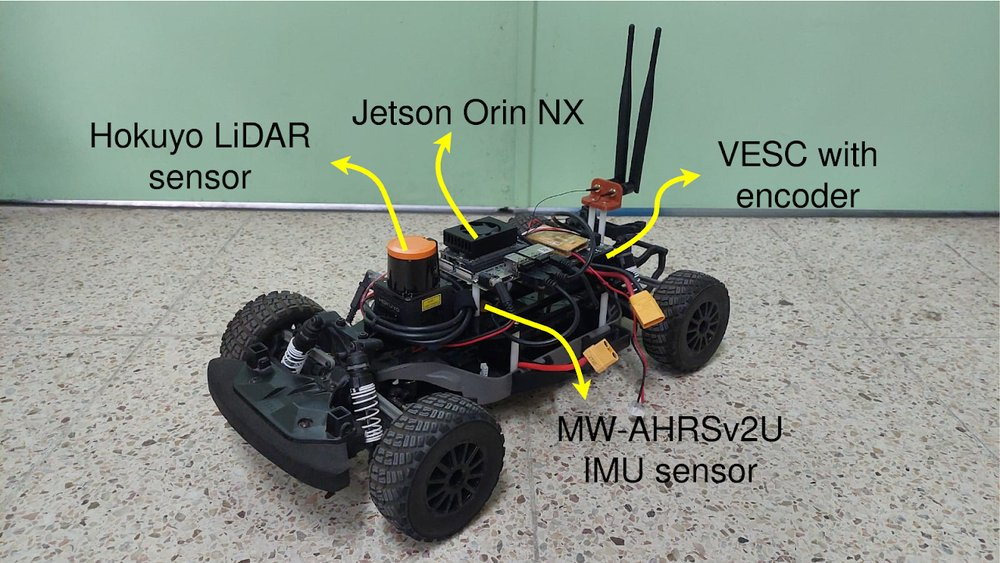
\includegraphics[width=\linewidth,height=0.6\textheight,keepaspectratio]{f1tenth_car.jpg}\\[8pt]
      {\scriptsize\color{textsec} F1TENTH platform}
    \end{column}
  \end{columns}
  \vfill
\end{frame}

\begin{frame}{Performance-Enhanced Risk-Aware MPPI using Gaussian Process\sectsuffix{Research}}
  \vfill
  \begin{columns}[c]
    \begin{column}{0.48\textwidth}\centering
      
\includegraphics[width=\linewidth,height=0.58\textheight,keepaspectratio]{p1_sim_w_obs}\\[8pt]
      {\scriptsize\color{textsec} Simulation --- with obstacles}
    \end{column}
    \begin{column}{0.48\textwidth}\centering
      
\includegraphics[width=\linewidth,height=0.58\textheight,keepaspectratio]{p1_sim_wo_obs}\\[8pt]
      {\scriptsize\color{textsec} Simulation --- without obstacles}
    \end{column}
  \end{columns}
  \vfill
\end{frame}

\begin{frame}{Performance-Enhanced Risk-Aware MPPI using Gaussian Process\sectsuffix{Research}}
  \blocklabel{Objective}
  Drive a robot safely despite the model--reality gap, without hand-tuning the safety level.
  \medskip
  \blocklabel{Outcome / Contribution}
  \begin{itemize}\small\setlength\itemsep{6pt}
    \item Gaussian Process learns the model gap offline and \textbf{auto-sets the safety level} --- no manual tuning.
    \item On F1TENTH (sim + real): finished every obstacle lap where baselines crashed, at the same speed.
  \end{itemize}
  \vfill

  \linkline{Images, video \& explanation}{https://gp-ramppi.github.io/}\\[3pt]
  \linkline{Paper (IEEE Access, 1st author)}{https://doi.org/10.1109/ACCESS.2025.3640166}
\end{frame}

\begin{frame}{Performance-Enhanced Risk-Aware MPPI using Gaussian Process\sectsuffix{Research}}
  \blocklabel{Technical skills}
  \begin{itemize}\setlength\itemsep{5pt}
    \item Gaussian Process
    \item MPPI / sampling MPC
    \item Localization \& mapping (SLAM)
    \item ROS1, move\_base (Nav2 equivalent), Gazebo
    \item PyTorch, PyCUDA
    \item Python, C/C++
    \item \textbf{Hardware:} Jetson Orin, LiDAR, IMU, wheel odometry, VESC
  \end{itemize}
\end{frame}

% ---------- SGP-MPPI ----------
\begin{frame}{Robust RA-MPPI using Online Learning\sectsuffix{Research}}
  \vfill
  \begin{columns}[c]
    \begin{column}{0.48\textwidth}\centering
      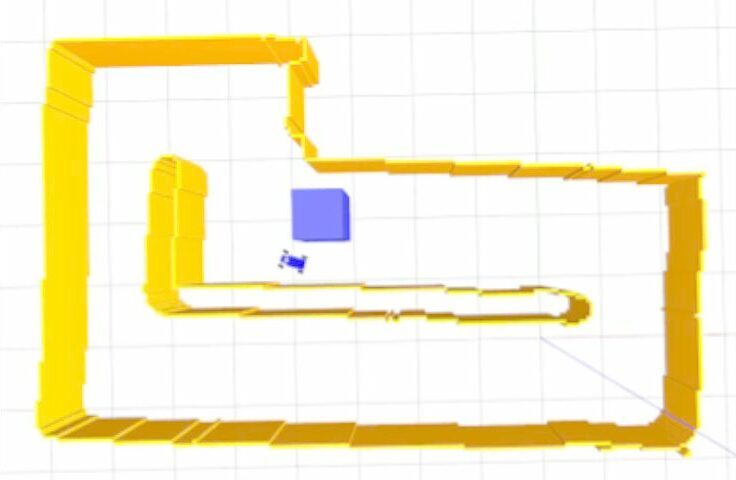
\includegraphics[width=\linewidth,height=0.58\textheight,keepaspectratio]{sgpmppi_sim_poster.jpg}\\[8pt]
      {\scriptsize\color{textsec} Simulation (Gazebo)}
    \end{column}
    \begin{column}{0.48\textwidth}\centering
      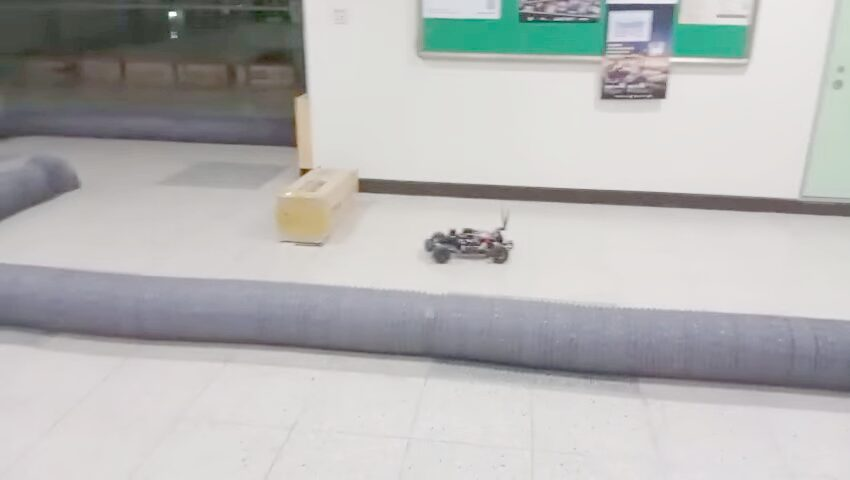
\includegraphics[width=\linewidth,height=0.58\textheight,keepaspectratio]{sgpmppi_real_poster.jpg}\\[8pt]
      {\scriptsize\color{textsec} Real-world run --- proposed method}
    \end{column}
  \end{columns}
  \vfill
\end{frame}

\begin{frame}{Robust RA-MPPI using Online Learning\sectsuffix{Research}}
  \vfill
  \begin{columns}[c]
    \begin{column}{0.5\textwidth}\centering
      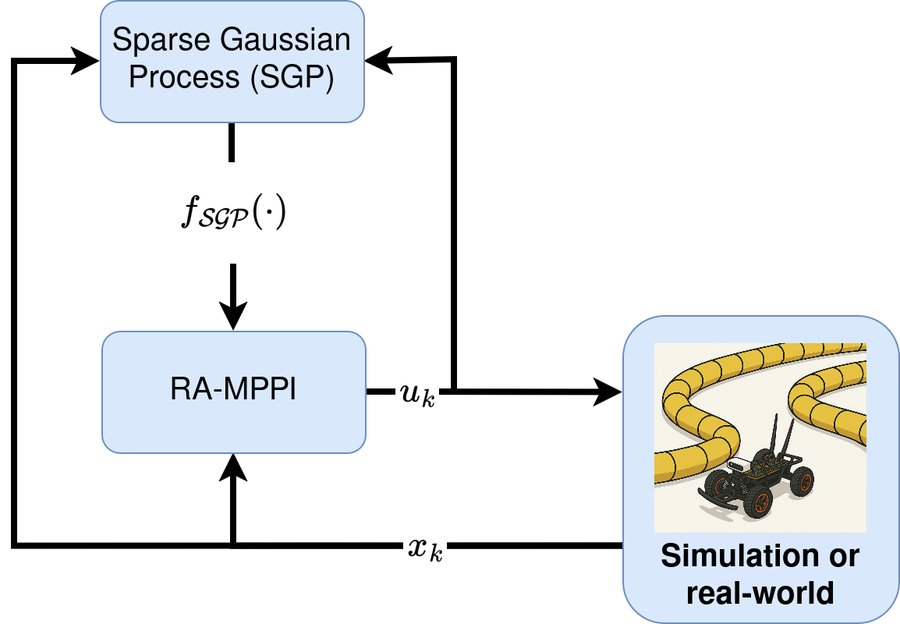
\includegraphics[width=\linewidth,height=0.6\textheight,keepaspectratio]{sgpmppi.jpg}\\[8pt]
      {\scriptsize\color{textsec} Control scheme}
    \end{column}
    \begin{column}{0.42\textwidth}\centering
      
\includegraphics[width=\linewidth,height=0.6\textheight,keepaspectratio]{p2_sampling}\\[8pt]
      {\scriptsize\color{textsec} Online sampling}
    \end{column}
  \end{columns}
  \vfill
\end{frame}

\begin{frame}{Robust RA-MPPI using Online Learning\sectsuffix{Research}}
  \blocklabel{Objective}
  Adapt to uncertainty in real time --- learn the model gap \textbf{while driving}, no data collected beforehand.
  \medskip
  \blocklabel{Outcome / Contribution}
  \begin{itemize}\small\setlength\itemsep{6pt}
    \item Sparse Gaussian Process learns the gap \textbf{online} in the background, never slowing control.
    \item On F1TENTH (sim, obstacles): \textbf{22 laps vs.\ 16} before, still real time.
  \end{itemize}
  \vfill

  \linkline{Images, video \& explanation}{https://sgp-mppi.github.io/}\\[3pt]
  {\footnotesize 1st author · Submitted to IJCAS (Springer)}
\end{frame}

\begin{frame}{Robust RA-MPPI using Online Learning\sectsuffix{Research}}
  \blocklabel{Technical skills}
  \begin{itemize}\setlength\itemsep{5pt}
    \item Sparse Gaussian Process (online learning)
    \item MPPI / sampling MPC
    \item Localization \& mapping (SLAM)
    \item ROS1, move\_base (Nav2 equivalent), Gazebo
    \item PyTorch, PyCUDA
    \item Python, C/C++
    \item \textbf{Hardware:} Jetson Orin, LiDAR, IMU, wheel odometry, VESC
  \end{itemize}
\end{frame}

% ========================================================
% ENGINEERING PROJECTS
% ========================================================
\section{Engineering Projects}

% ---------- ESP32 IoT Medical Gateway ----------
\begin{frame}{ESP32 IoT Medical Gateway\sectsuffix{Engineering Projects}}
  \vfill
  \begin{center}
    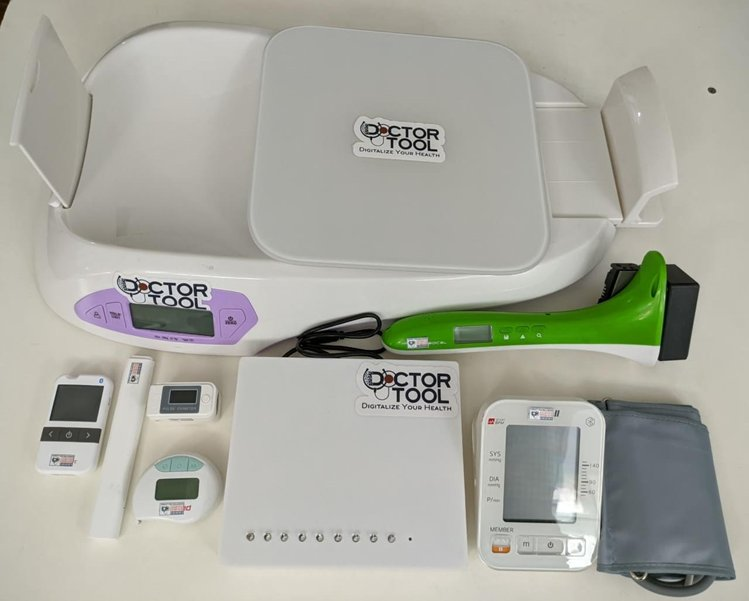
\includegraphics[height=0.66\textheight,keepaspectratio]{iotm.jpg}
  \end{center}
  \vfill
\end{frame}

\begin{frame}{ESP32 IoT Medical Gateway\sectsuffix{Engineering Projects}}
  \blocklabel{Objective}
  Connect medical instruments to the cloud for posyandu (community health post) measurements.
  \medskip
  \blocklabel{Outcome / Contribution}
  \begin{itemize}\small\setlength\itemsep{6pt}
    \item Built an ESP32 gateway linking thermometers, oximeters, and biometric sensors.
    \item Connected over six categories of medical devices.
  \end{itemize}
  \vfill
  {\footnotesize\color{textsec} Internship at DoctorTool \,\textbullet\, Team of 2 \,\textbullet\, 2022}
\end{frame}

\begin{frame}{ESP32 IoT Medical Gateway\sectsuffix{Engineering Projects}}
  \blocklabel{Technical skills}
  \begin{itemize}\setlength\itemsep{6pt}
    \item Embedded / IoT
    \item RTOS (FreeRTOS)
    \item BLE connectivity
    \item Reverse engineering
    \item C/C++
    \item \textbf{Hardware:} ESP32
  \end{itemize}
\end{frame}

% ---------- 6-DOF Robot Manipulator ----------
\begin{frame}{6-DOF Robot Manipulator Simulation (OpenGL)\sectsuffix{Engineering Projects}}
  \vfill
  \begin{center}
    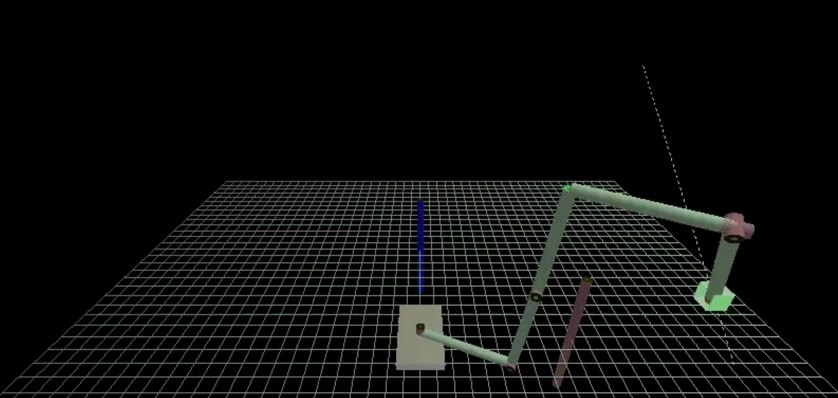
\includegraphics[height=0.66\textheight,keepaspectratio]{robot6dof.jpg}
  \end{center}
  \vfill
\end{frame}

\begin{frame}{6-DOF Robot Manipulator Simulation (OpenGL)\sectsuffix{Engineering Projects}}
  \blocklabel{Objective}
  Visualize and control a 6-DOF robot arm in real time.
  \medskip
  \blocklabel{Outcome / Contribution}
  \begin{itemize}\small\setlength\itemsep{6pt}
    \item Real-time 3D arm in C/OpenGL with forward and Jacobian-pseudoinverse IK.
    \item Point-to-point trajectories, joint commands streamed over serial.
  \end{itemize}
  \vfill
  {\footnotesize\color{textsec} Course project \,\textbullet\, Universitas Indonesia \,\textbullet\, May 2023}\\[3pt]
  \linkline{Source code}{https://github.com/hanifedma/robot-6dof-opengl}
\end{frame}

\begin{frame}{6-DOF Robot Manipulator Simulation (OpenGL)\sectsuffix{Engineering Projects}}
  \blocklabel{Technical skills}
  \begin{itemize}\setlength\itemsep{6pt}
    \item C
    \item OpenGL / GLUT
    \item Robot kinematics (FK/IK)
    \item MATLAB
    \item Robotics Toolbox (Peter Corke, MATLAB)
  \end{itemize}
\end{frame}

\end{document}
